\documentclass[a4paper]{report}
\usepackage{tikz}
\usepackage[margin=2.5cm]{geometry}
\usepackage{hyperref}
\usepackage{graphicx}
\graphicspath{{figures/}{anotherFigureDirectory/}}
\graphicspath{ {./images/} }
\usepackage{listings}
\usepackage{wrapfig}
\usepackage{color}
\definecolor{bluekeywords}{rgb}{0.13,0.13,1}
\definecolor{greencomments}{rgb}{0,0.5,0}
\definecolor{turqusnumbers}{rgb}{0.17,0.57,0.69}
\definecolor{redstrings}{rgb}{0.5,0,0}
\definecolor{gray}{rgb}{0.13,0.13,0.13}
\lstdefinelanguage{FSharp}
                {morekeywords={let, new, match, with, rec, open, module,
                namespace, type, of, member, and, for, in, do, begin, end, fun,
                function, try, mutable, if, then, else},
                keywordstyle=\color{bluekeywords},
                sensitive=false,
                numbers=left,  % where to put the line-numbers;(none, left, right)
                numberstyle=\tiny\color{gray},
                morecomment=[l][\color{greencomments}]{///},
                morecomment=[l][\color{greencomments}]{//},
                morecomment=[s][\color{greencomments}]{{(*}{*)}},
                morestring=[b]",
                showstringspaces=false,
                stringstyle=\color{redstrings}
                }

\title{PoP - Ugeopgave 7}
\author{Christoffer, Inge og Pernille}
\date{\today}

\begin{document}
\maketitle
\tikzstyle{block} = [rectangle, draw, fill=blue!20, text centered,
    rounded corners, minimum height=2.5em]
\tikzstyle{cloud} = [rectangle, draw, fill=white, text centered,
    rounded corners, minimum height = 2em]
\tikzstyle{line} = [draw, -latex]

\section*{Preface}
As a part of the Programming and Problem Solving course, we,
three Computer Science students at Copenhagen University, build the game Awari.

\section*{Awari}
Awari is an ancient two player game that resembles the beloved Kalaha. The main
objective of Awari is to capture the most beans. The game consists of a board
with 6 pits and one home pit for each player. Each of the 6 x 2 pits contain
3 beans. The players must in turn take the amount of beans from a pit on their
side of the board and distribute them in the following pits. The game
continues until one of the two players has no beans left, and the winner is the
player who captured the most beans in their homepit.

\section*{Problem description}
We have implemented Awari using the functional programming language F\#. We
were given two functions as a start, a turn and a play function, and a signature
file with type indications for several minor functions. To be able to play the
game we have created functions to print the board, to distribute the beans, to
check for game over etc. All the functions will be elaborated in this rapport.

\begin{figure}
\centering
\begin{tikzpicture} [node distance = 1.5 cm, auto]
		\node [cloud] (start) {The board is printed};
        \node [cloud, below of=start] (choise) {A player chooses a pit};
        \node [cloud, below of=choise] (distribute) {Beans are distributed};
        \node [cloud, below of=distribute] (eval) {The result is evaluated};
		\node [cloud, right of=eval, node distance = 4.5 cm]
            (newp) {Retry or change of turns};
        \node [cloud, left of=eval, node distance = 4 cm]
            (end) {The game is over};
        % Arrows
        \path [line] (start) -- (choise);
        \path [line] (choise) -- (distribute);
        \path [line] (distribute) -- (eval);
        \path [line] (eval) -- (newp);
        \path [line] (newp) |- (start);
        \path [line] (eval) -- (end);

\end{tikzpicture}
\caption{Flow of Awari}
\label{fig:gameflow}
\end{figure}

\section*{Problem analysis and design}
\subsection*{Gameboard and flow}
We designed our program starting by focusing on the gameboard. The board is
the center of the game and thus the main part of our functions takes the board
as input and returns a new board or evaluates the pits at the board. Figure 1
illustrates the simple flow of the game. The board with the correct number of beans in each of the pit is the starting point. In the real physical game, you start by setting op the game board to play by putting beans in the pits. The virtual counterpart is printing the board. Hereafter, the players start playing beginning with Player1 picking a pit. As we see from Figure
\ref{fig:gameflow}), the player returns to the printed board after every turn. Based on this, we started by creating our board. It consists of an int array with 14
integers where two are home pits and six pits for each player. As an array
is mutable we preferred this type to lists.

\subsection*{Design and user interface}
The design of the gameboard was important to us. We wanted the gui design to be nice, simple and intuitive to the player. Therefore we started by focusing on the
\texttt{printBoard} function.

\begin{wrapfigure}{r}{0.75\textwidth}
\centering
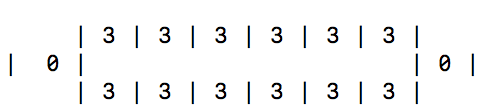
\includegraphics[width=0.60\textwidth]{board1}
\caption{Board of Awari}
\end{wrapfigure}
Prints the array formed as a gameboard. This makes it clear to the player that it is a gameboard an not just an array of integers. All the pits are clearly divided and the homepits are situated at each end of the board. We thought that the screen got cluttered with the compiling code and all the printed boards. Therefore we added the \texttt{System.Console.Clear} function to make the terminal look more as a game screen.
\newline
\begin{wrapfigure}{l}{0.75\textwidth}
\centering
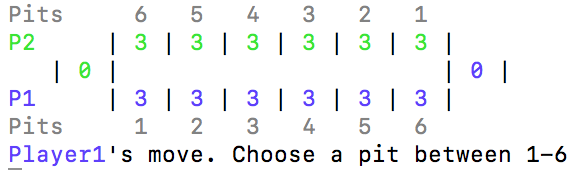
\includegraphics{boardcolor}
\caption{Board of Awari with colour}
\end{wrapfigure}

We still suspected that the players could be confused about which pits and
which side of the board belonged to who. Therefore we added colours to the
pits and the players: Player 1 is blue and has the blue pits. Player 2 is green
 and has the green pits. In addition, we added the numbers of the pits so to
not to get confused of which pit is which and in which direction the game is played.

\subsection*{The Players}
The game is played by two players. We have created a type player consisting of a player1 and player2. It is important to distinguish between the two as they have each their home pit and each their side of the board, meaning that they have a specific index as their pits. Player1 has index 0-5 and has homepit in index 6. Player2 has index 7-12 and homepit in index 13. To solve this issue, we made a function \texttt{isHome} that was able to recognize which homepit belonged to each of the players.

We also needed to know the player's choice of pit from which he or she wanted to take beans. We decided that it should be possible for each player to enter a number on the keyboard between 1-6 and then the game had to convert it to the correct index number, instead of just letting the player know which index numbers belong to him or her. We created the function \texttt{getMove} to solve this problem. It matches the player and the input from a pressed keyboard and returns an index.

\subsection*{Playing the game}

Another function we focused on was the \texttt{distribute}
function as it distributes the beans taken from a pit and placed in the following. Thereby it updates the board and secure the flow in the game.
\begin{wrapfigure}{l}{0.9\textwidth}
\centering
\begin{tikzpicture} [node distance = 1.5 cm, auto]
		\node [cloud] (start) {3-3};
        \node [cloud, below of=start] (choise) {3+1};
        \node [cloud, below of=choise] (distribute) {2+1};
        \node [cloud, below of=distribute] (eval) {0+1};
		\node [cloud, right of=eval, node distance = 4 cm]
            (newp) {if Home, try again};
        \node [cloud, left of=eval, node distance = 4 cm]
            (end) {If empty, check opposite};
        % Arrows
        \path [line] (start) -- (choise);
        \path [line] (choise) -- (distribute);
        \path [line] (distribute) -- (eval);
        \path [line] (eval) -- (newp);
        \path [line] (eval) -- (end);

\end{tikzpicture}
\caption{Example of the distribute function}
\end{wrapfigure}
\\\\
\\\\
\\\\
\\\\
\\\\
\\\\
\\\\
\\\\
\\\\
Figure 4 illustrates an example of the distribute function, where it takes the 3 beans from the chosen pit and places them in the following. It is a bit more complex than this which is elaborated in the section about functions.

\section*{Program description}
\subsection*{Types}
From the assignment we've been given some essential types, which were needed to set some game-specified types used in nearly every single game function.

\lstset{language=FSharp}
\lstinputlisting{types.fsx}

\subsubsection*{board}
The type \texttt{board} takes the fsharp-type \textsl{int array} and is used to create the board of the game representing 12 general pits and 2 homepits, i.e. at set of 6 generals and 1 home per. player.

\subsubsection*{player}
The type \texttt{player} is simply created to make it possible for a function to take the type as an argument. The type has two possible versions \textsl{Player1} or \textsl{Player2}.

\subsubsection*{pit}
Finally the type \texttt{pit} is given the type integer, and was created quite like \texttt{player}, to make it possible for future functions to take a pit number, representing an index number in the given board array, as an argument.

\subsection*{Globals}
For showing the colours of players and their pits at the printed game board, we have defined \texttt{player1Color} and \texttt{player2Color}. We use \texttt{pitNumberColor} as the colour of the pits numbers, and \texttt{gameOverColor} is used when the game terminates it write Game Over.
\\\\
We have also defined beginning board, \texttt{board}, with the type array.

\subsection*{makeSpaces}
{\it This function is used to make making several spaces in a string more simple.}
\lstinputlisting[language=FSharp, firstline=25, lastline=29]{AwariLib.fs}
The function takes an integer as it sole argument, used to determine the number of spaces one wishes to implement, and returns a string of spaces corresponding to the given int input.

\subsection*{addColor}
{\it This function is used to add color to text printed in the terminal.}
\lstinputlisting[language=FSharp, firstline=40, lastline=42]{AwariLib.fs}
The function takes two arguments: a string and integer. The string input represents the string one wishes to apply a text color to, and the integer represents a color corresponding to a color value in the ANSI
It uses the ANSI escape sequence which, amongst other features, can be used to control the color of the text in the terminal. By using the sequences Esc and '[', we are able to make the terminal interpret the sequence as a command instead of just characters of code. This is why we need to define the varable \texttt{esc} in the function. The function then includes a \texttt{sprintf} statement where the \texttt{esc} variable and color value is applied to the given string.

\subsection*{makeP1Field \& makeP2Field}
{\it These functions use \texttt{addColor} and \texttt{makeSpaces} and are used to created and color the pits of each player respectively.}
\lstinputlisting[language=FSharp, firstline=51, lastline=57]{AwariLib.fs}
\lstinputlisting[language=FSharp, firstline=66, lastline=72]{AwariLib.fs}
The functions \texttt{makeP1Field} and \texttt{makeP2Field} takes a given board as it's sole argument and returns af string of pipes and numbers representing the pits of \texttt{Player1} and \texttt{Player2} respectively. By use of a \texttt{for}-loop, the function concatenates 6 strings made up of the value held by the given index in the board array and a pipe, used as a visual separator between each pit.


\subsection*{makeHomes}
{\it This function uses \texttt{addColor} and \texttt{makeSpaces} and creates the home pits of both players.}
\lstinputlisting[language=FSharp, firstline=81, lastline=86]{AwariLib.fs}
The function \texttt{makeHomes} takes a given board as it's argument and returns a string representing the home pits of \texttt{Player1} and \texttt{Player2}. By creating a mutable empty string we were then able to concatenates the final home pits string made up of the values held by the given indexes in the board array corresponding to the two home pits.


\subsection*{makeP1PitNumbers \& makeP2PitNumbers}
{\it These functions use \texttt{makeSpaces} and are used to created and color the pits of each player respectively.}
\lstinputlisting[language=FSharp, firstline=94, lastline=97]{AwariLib.fs}
\lstinputlisting[language=FSharp, firstline=105, lastline=108]{AwariLib.fs}
The functions \texttt{makeP1PitNumbers} and \texttt{makeP2PitNumbers} takes no arguments and returns a string of numbers representing the number between 1 and 6 referring to the corresponding pit of each player. 

\subsection*{printBoard}
{\it This functions uses \texttt{addColor}, \texttt{makeP2PitNumbers}, \texttt{makeP2PitNumbers}, \texttt{pitNumberColor}, \texttt{player1Color}, \texttt{player2Color}, \texttt{makeP1Field}, \texttt{makeHomes} \texttt{makeP2Field} and is used to creat the current game board.}
\lstinputlisting[language=FSharp, firstline=126, lastline=134]{AwariLib.fs}
The function \texttt{printBoard} takes a given board as it's sole argument and returns the current game board by use of several of the supporting functions described in the above sections. By creating a mutable empty string, as with \texttt{makeHomes}, we were able to then concatenates the fields and homes of both players, made up of the values held by each index in the board array and the injected pipes and spaces separating the pit and home pit values.

\subsection*{isGameOver}
{\it This function is used by \texttt{turn} and \texttt{play}.}
\lstinputlisting[language=FSharp, firstline=143, lastline=147]{AwariLib.fs}
The function takes a board as input and returns a boolean. It returns true if either side of the board has no beans. It is called by \texttt{turn} to check whether the game is over, if it returns True, the whole game terminates.

\subsection*{isHome}
{\it This function is used by \texttt{turn}.}
\lstinputlisting[language=FSharp, firstline=160, lastline=164]{AwariLib.fs}
The function checks whether a given pit is the homepit for one of the players. It is a boolean type and returns true if it is so.
It is called by \texttt{turn} to a given board, the finalPitsPlayer and the finalPit. If it does not return true in this context, \texttt{turn} returns a new board and the game continues. Else, it calls \texttt{repeat} again with the same player.

\subsection*{getMove}
{\it This function gets a player's next move.}
\lstinputlisting[language=FSharp, firstline=176, lastline=195]{AwariLib.fs}
The function uses \texttt{System.Console.Readline} to get a keyboard input and then translates this to a pit number. It is only possible for the player to choose between 1-6. If another key is entered, the player is asked to try again. The function matches the player with the input to make sure to return a valid pit in consistence with the player.

\subsection*{checkOpp}
{\it This function checks whether there are any beans in the opposite pit of the final pit.}
\lstinputlisting[language=FSharp, firstline=208, lastline=213]{AwariLib.fs}
\texttt{checkOpp} is of type boolean and returns true if there are beans in the opposite pit from the final pit. If the opposite pit is any of the home pits, or if the opposite pit contains zero beans, then it returns false. \texttt{checkOpp} is used by the function \texttt{distribute} to take the beans from the opposite pit to the home pit if the final pit is empty.

\subsection*{finalPitPlayer}
{\it This function returns the player of the final pit.}
\lstinputlisting[language=FSharp, firstline=223, lastline=226]{AwariLib.fs}
If the final pit is less or equal to 6, \texttt{finalPitPlayer} returns player 1. Else it returns player 2. The function is used in the \texttt{distribute} function.

\subsection*{distribute}
{\it This function distributes the beans from the chosen pit counter clockwise}
\lstinputlisting[language=FSharp, firstline=239, lastline=262]{AwariLib.fs}
\texttt{distribute} is one of the key function in the game as already described. It sets a variable k equivalent to the number of beans in the chosen pit i. It then uses a while loop to distribute the number of beans k in the following pits, j, by adding one to b.[j] while taking one from k by each distribution. It then updates the finalPit to be j and checks whether there are any beans in the pit opposite the end pit. If so, the function adds them to the home pit and then updates the final pit and the opposite pit to be zero. At the end it returns a tuple containing of the updated board, the final pit player and the final pit. \texttt{distribute} is called by the \texttt{turn} function.

\subsection*{playerAsString}
{\it This function is created to convert the type \texttt{player} to the type \texttt{string}}
\lstinputlisting[language=FSharp, firstline=265, lastline=268]{AwariLib.fs}
The function \texttt{playerAsString} takes the type \texttt{player} as it's argument and returns a string corresponding to the relevant player input. Such that p = \texttt{Player1} returns the string "Player1" and p = \texttt{Player2} returns the string "Player2".

\subsection*{turn}
{\it The function evaluates the turn of a player}
\lstinputlisting[language=FSharp, firstline=279, lastline=294]{AwariLib.fs}
\texttt{turn} is another key function of the programme. It was handed  to us from the beginning, but we have altered it slightly. It contains a recursive function \texttt{repeat} that gets the player, the board and the entered 	pit number from \texttt{getMove} to evaluate who's turn it is and returns the new board. It calls for \texttt{printBoard} to print the board and then it call for \texttt{playerAsString} to let the players know who's turn it is.
Then it makes three variables, newB, finalPitsPlayer and finalPit and updates them via a call to \texttt{distribute} to the board, the player and i. i is a pit number retrieved from a call to \texttt{getMove}.
Then the function checks if the final pit is not the player's home (it calls for \texttt{isHome}), or if the game is over (it calls for \texttt{isGameOver}) and then it returns a new board, newB. Else the \texttt{repeat} function calls itself as it is the same player again. Then it calls itself to the new player.

\subsection*{play}
{\it The only function called in the application file}
\lstinputlisting[language=FSharp, firstline=306, lastline=324]{AwariLib.fs}
The \texttt{play} function is the only function that is called in the application file. It was also a piece of code that was handed to us but we have altered it some.
At first, it asks if the game is over as it calls \texttt{isGameOver}. If true, it prints the board and announces the winner. We have added the winner announcement to the function. If the game is not over jet, it returns a new board newB that calls for \texttt{turn}, and the next player nextP. Then it calls itself recursively to newB and newP.
\\
\section*{Testing}
We tested the functions using the princinples of whitebox testing. We encountered difficulties with some of the functions, as they were not returning any comparable value or relied on a user input.
We decided to alter the functions that relied on user input. All tests can be performed using the Whiteboxtest.fsx. Details on the branches will be printed when performed.

\subsection*{getMove}
getMove is one of the functions that had to be altered for proper testing. Instead of using n as the input based on a System.Console.ReadLine(), we created a new parameter called key.
We could then use key to test different user inputs.
\lstinputlisting[language=FSharp, firstline=110, lastline=132]{Whiteboxtest.fsx}

\subsection*{turn}
turn is the other function that had to be altered. Using the same principle we used the parameter move in place of the System.Console.ReadLine() to enable use to do the testing of the function. The function would then use move
to return a new board.
\lstinputlisting[language=FSharp, firstline=178, lastline=193]{Whiteboxtest.fsx}

\section*{Discussion}
We created Awari using only functional programming. The game fulfills the requirements. We encountered several problems regards the playability of the game. We wanted a game that could be with little to none
instructions. We tried to make it more clear to the user which pits that were Player1s and which that were Player2s, using colors.
\section*{Appendix}
\lstset{language=FSharp}
\lstinputlisting{AwariLib.fs}
\end{document}
